% Suggested captions for the shift-experiment figures (numbers regenerate with: python -m telo_tabular.make_figures --root runs_shift --out figures)

\begin{figure*}[t]
\centering
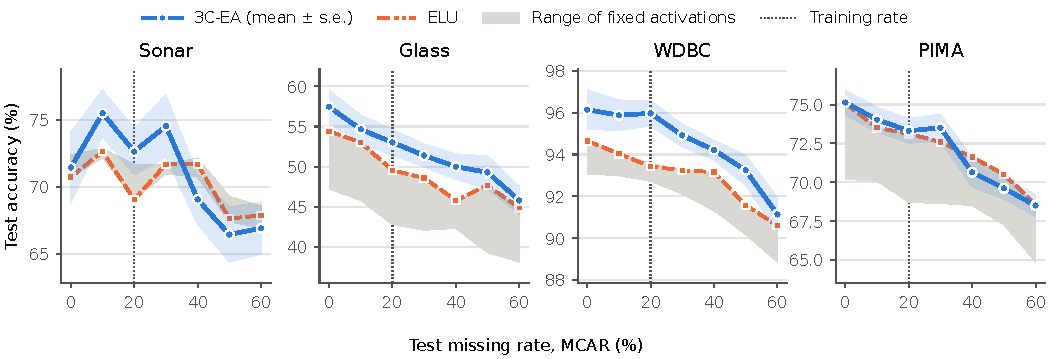
\includegraphics[width=\linewidth]{figures/fig_shift_curves.pdf}
\caption{Test accuracy when the test missing rate differs from training. All models are trained at 20\% MCAR
(dotted line) and evaluated without retraining at MCAR rates from 0\% to 60\%; imputation statistics and confidence
values are frozen from training. The blue line is 3C-EA (mean over runs, band $\pm$ one standard error), the dashed
line is ELU, and the grey band spans the means of the four fixed activations (ReLU, Swish, LeakyReLU, ELU).
Vertical axes differ between panels.}
\label{fig:shift-curves}
\end{figure*}

\begin{figure*}[t]
\centering
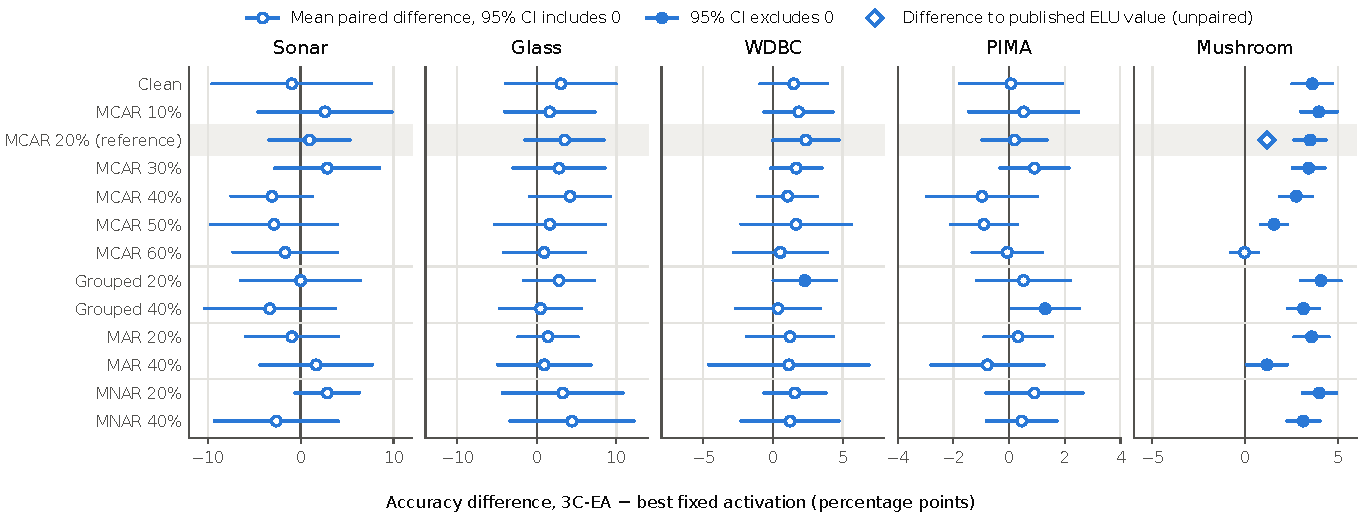
\includegraphics[width=\linewidth]{figures/fig_shift_differences.pdf}
\caption{Paired accuracy difference between 3C-EA and the best fixed activation under each test condition, for models
trained at 20\% MCAR (shaded row) and frozen. The best fixed activation is chosen separately for every condition by
its mean, which favours the baseline. Points are means over runs with identical splits and masks; bars are 95\%
$t$-intervals of the paired difference. Filled points mark intervals that exclude zero; no correction for multiple
comparisons is applied. Horizontal axes differ between panels.}
\label{fig:shift-differences}
\end{figure*}

\begin{figure*}[t]
\centering
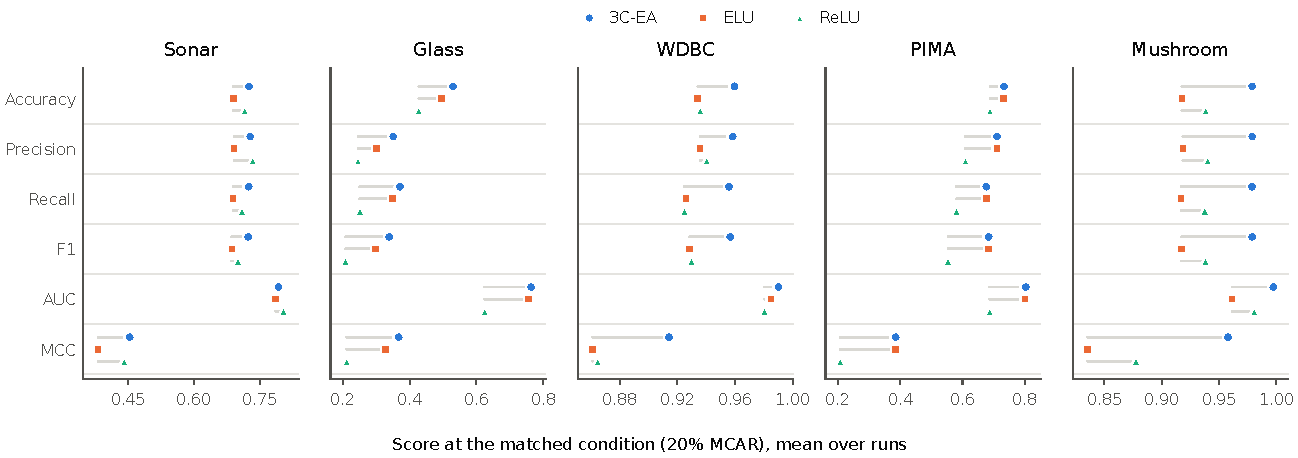
\includegraphics[width=\linewidth]{figures/fig_matched_metrics.pdf}
\caption{Six evaluation measures at the matched condition (trained and tested at 20\% MCAR), mean over runs.
Precision, recall and F1 are macro-averaged; AUC is one-vs-rest for the multi-class Glass dataset; MCC is the
Matthews correlation coefficient. Horizontal axes differ between panels.}
\label{fig:matched-metrics}
\end{figure*}

\begin{figure}[t]
\centering
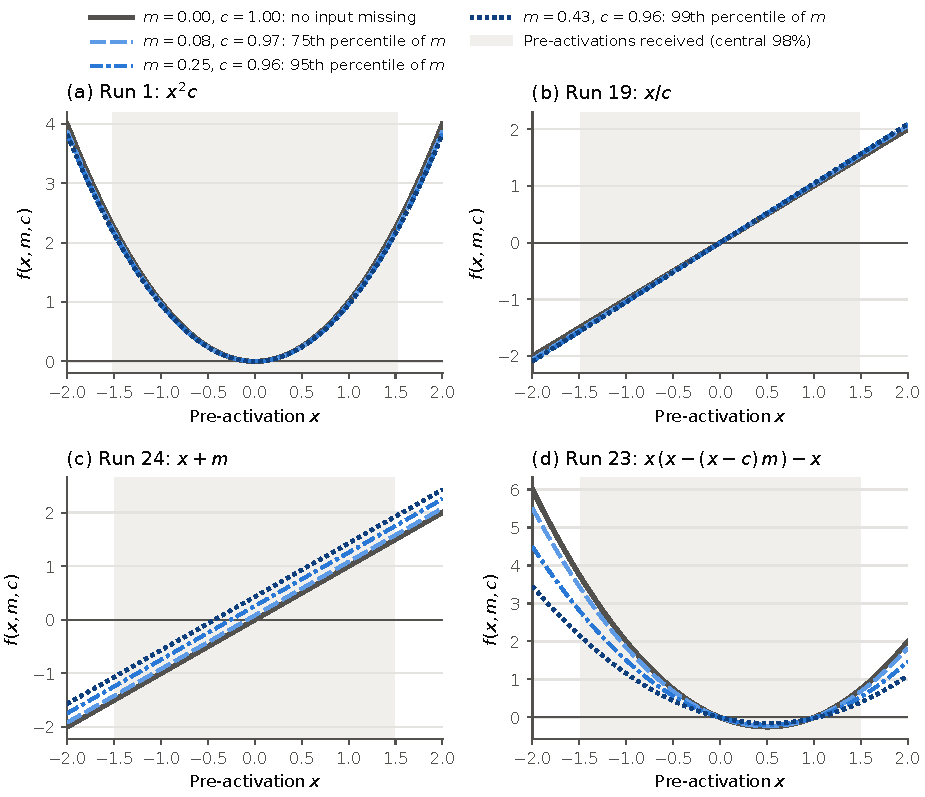
\includegraphics[width=\linewidth]{figures/fig_response_examples.pdf}
\caption{Evolved activation functions drawn at the missingness $m$ and confidence $c$ that reach the first hidden layer.
Each function was trained on 30 splits of its dataset; a line is one reliability state, given by a percentile of the
propagated $m$ over all unit--record pairs together with the $c$ that accompanies it, and the grey band is the central
98\% of the pre-activations received. (a)~A function evolved on Cylinder Bands: the response becomes about twice as
steep between the 5th and the 99th percentile. (b)~The same function retrained on 100 new splits with both channels,
compared with itself when $c$ is fixed to 1 ($m$ only), $m$ is fixed to 0 ($c$ only) or both are fixed, and with the best
fixed activation; points are mean paired differences, bars are 95\% $t$-intervals, and filled points mark intervals that
exclude zero. (c,\,d)~Runs 24 and 23 of Table~\ref{tab:winners}, evolved on Hepatitis, where $m$ shifts or reshapes the
response by up to 29\% and 42\% of its largest fully observed value within the band.}
\label{fig:response-examples}
\end{figure}
